\documentclass[../../../main]{subfiles}
\begin{document}

\section{考察}

\subsection{アモルファス太陽電池とシリコンフォトダイオードの電流出力}
アモルファス太陽電池の分光感度特性は、波長が約\SI{400}{\nano m}から約\SI{800}{\nano m}までの光を吸収し、一般にピークは\SI{500}{nm}から\SI{600}{nm}の範囲にある\cite{evaluation-photo,amorfous-si}(図\ref{subfig:bunkoukando})。
シリコンフォトダイオードの分光感度特性は、一般に\SI{400}{\nano m}から約\SI{1000}{\nano m}までの光を吸収し、ピークは\SI{800}{nm}から\SI{900}{nm}の範囲にある(図\ref{subfig:solarcell})。
\begin{figure}
	\centering
	\begin{subfigure}{0.3\linewidth}
		\centering
		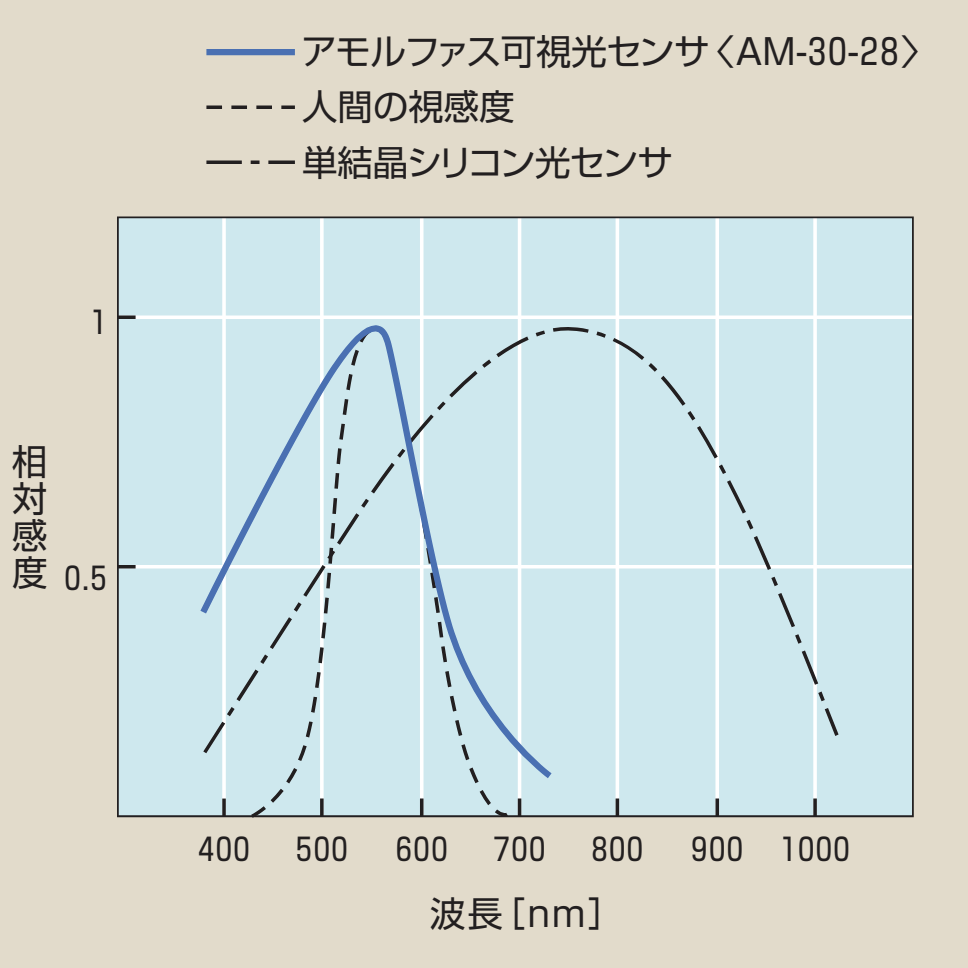
\includegraphics[width=0.9\linewidth]{src/figures/consi1/photodiode.png}
		\subcaption{フォトダイオードの分光感度特性\cite{amorfous-si}}\label{subfig:bunkoukando}
	\end{subfigure}
	\begin{subfigure}{0.6\linewidth}
		\centering
		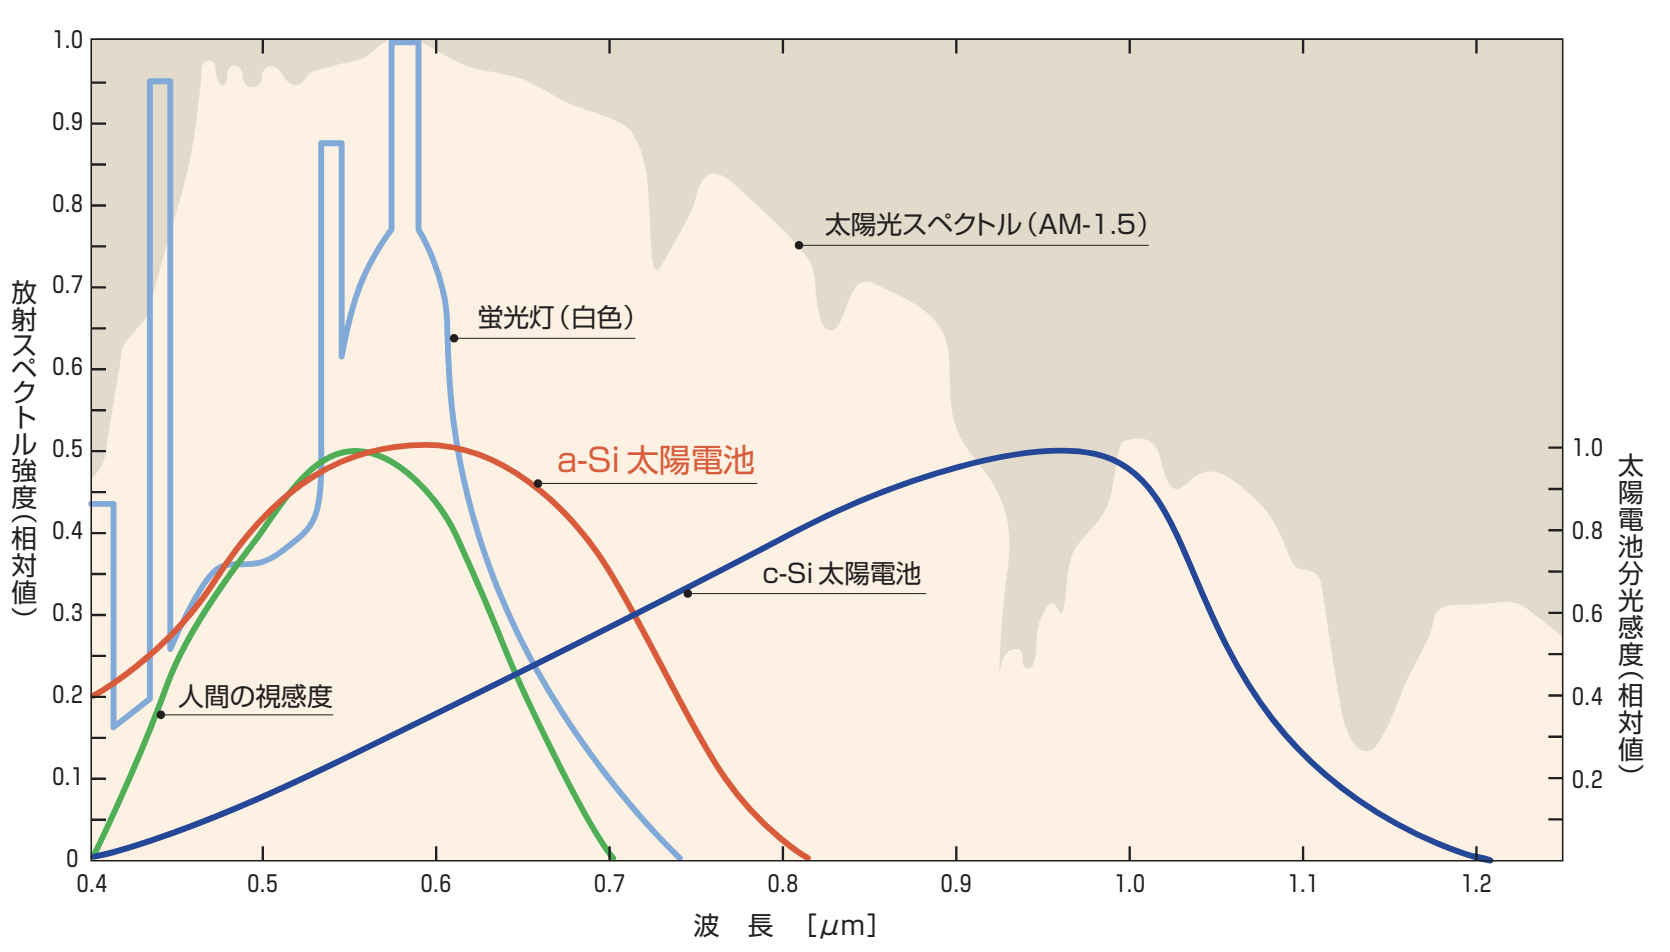
\includegraphics[width=0.9\linewidth]{src/figures/consi1/solarcell.png}
		\subcaption{太陽電池の分光感度特性\cite{amorfous-si}}\label{subfig:solarcell}
	\end{subfigure}
	\caption{太陽電池とフォトダイオードの分光感度特性}\label{fig:bunkoukando}
\end{figure}

蛍光灯、LEDライト、MAGライト(白色電球)のスペクトルは、次の図\ref{fig:wave-inte}のようになっている\cite{spectra}。
\begin{figure}
	\centering
	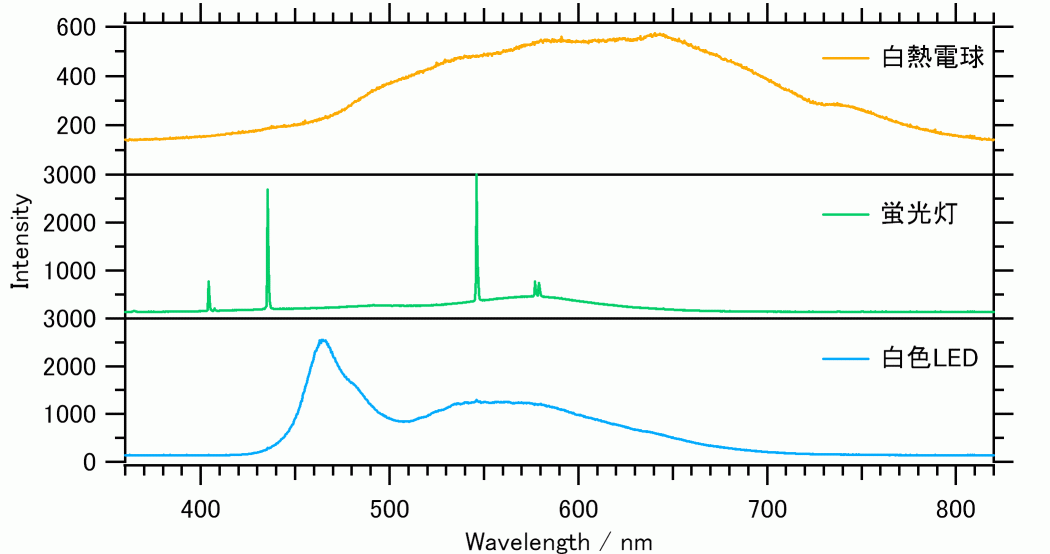
\includegraphics[width=0.6\linewidth]{src/figures/consi1/wave-inte.png}
	\caption{さまざまな光におけるスペクトル}\label{fig:wave-inte}
\end{figure}

このスペクトルと分光感度特性と表\ref{tab:exp1}を比較する。
まずアモルファス太陽電池についてはLEDライト照射時に最大となっている。
これは、アモルファス太陽電池の分光感度特性のピークが\SI{500}{nm}前後にピークがあり、LEDライトのスペクトルのピークは\SI{450}{nm}前後にあるためより効率的に光を吸収していると考えられる。
一方でシリコンフォトダイオードは、MAGライトが最大となっている。
これはシリコンフォトダイオードの分光感度が\SI{400}{nm}から\SI{1000}{nm}の範囲で鈍いピークをもっており、MAGライトのスペクトルも同様に\SI{400}{nm}から\SI{800}{nm}の範囲で幅広い鈍いピークをもっているためと考えられる。

\subsection{VPSの出力特性}\label{subsec:consi-vps}
図\ref{fig:exp2}に近似曲線を当てはめたものを図\ref{fig:vps-dmm-with-fit}に示す。
近似曲線の式は$A_{real}=0.996A_{conf}+0.024$となった。
ほとんど設定値と実測値は一致していると言えるが、表\ref{tab:exp2}より\SI{0.4}{A}未満では\SI{0.33}{A}でほぼ一定であり設定値と計測値がずれている。
したがって、これらを除いて\SI{0.4}{A}以上の範囲で近似曲線は$A_{real}=1.00A_{conf}-0.010$となり、設定値と実測値がほぼ一致した。
以上より、\SI{0.4}{A}以上では上記の近似曲線によって設定値と実測値を結びつけることができ、\SI{0.4}{A}未満では設定値と実測値がずれており約\SI{0.3}{A}になっていると考えられる。
以後はDMMによる計測結果が正しいとして、設定電流に対して以上のような出力が得られると考える。
\begin{figure}[!htb]
	\centering
	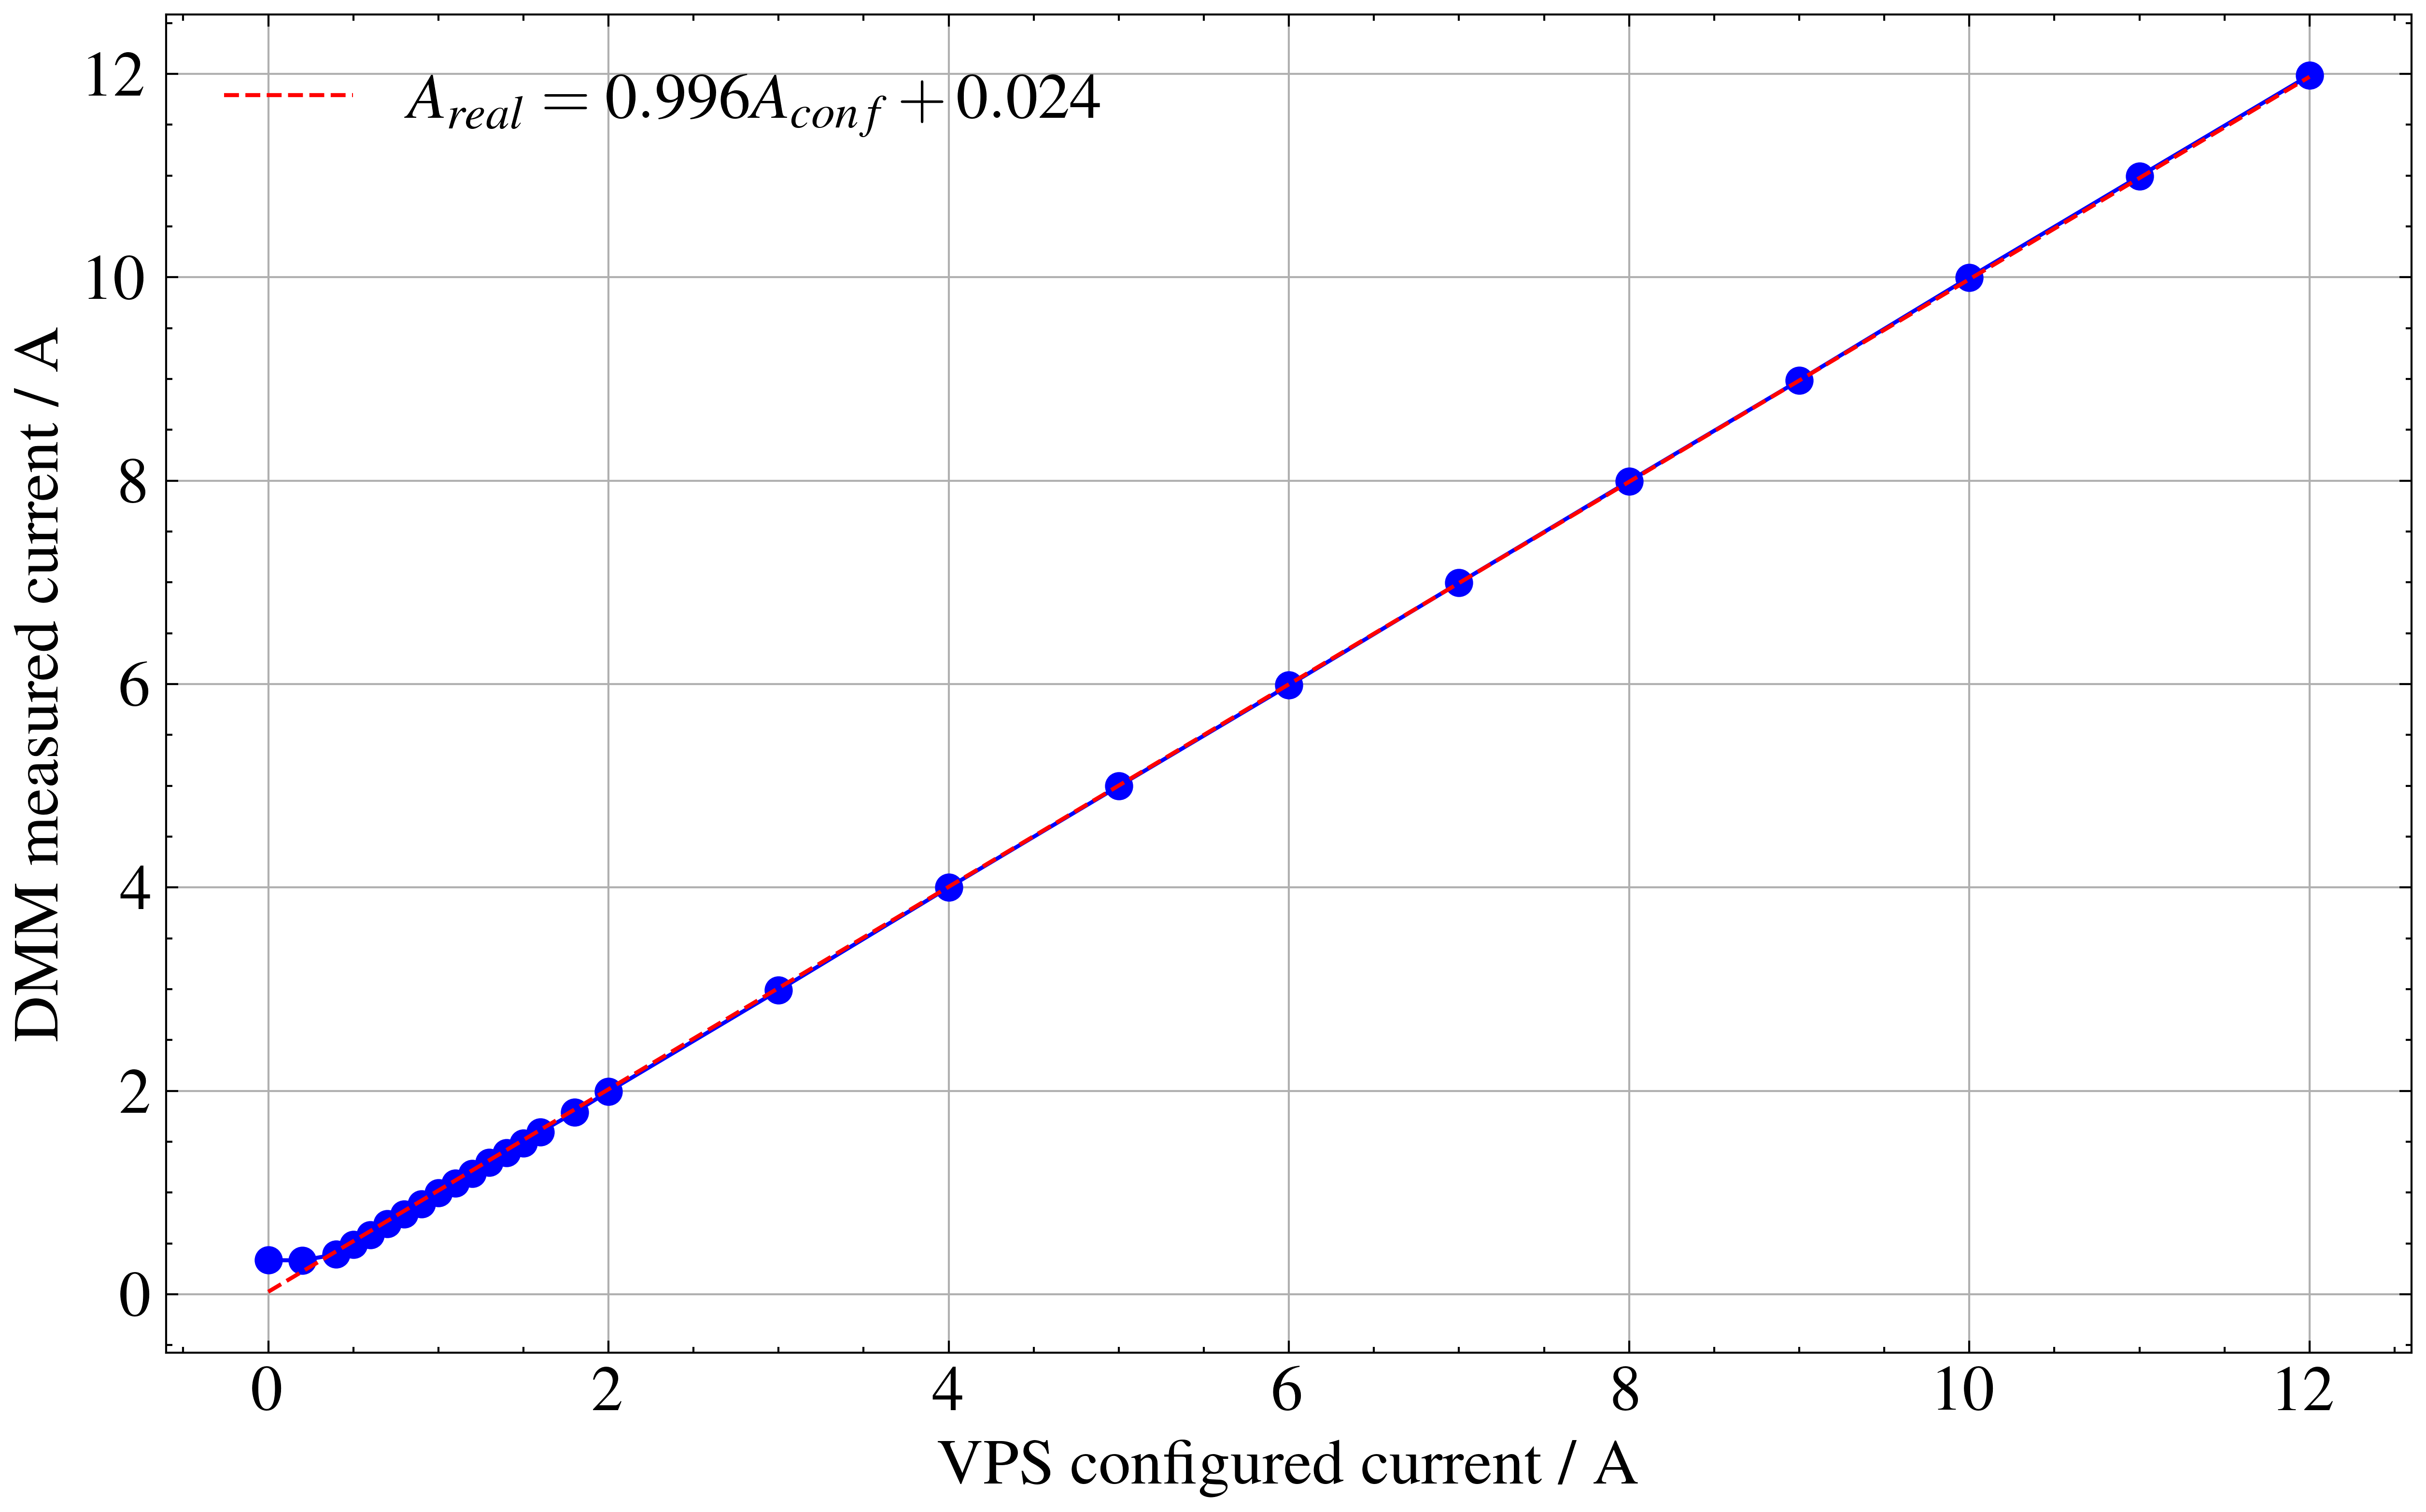
\includegraphics[width=0.6\linewidth]{src/figures/consi2/vps-dmm-with-fit.png}
	\caption{VPSの出力特性}\label{fig:vps-dmm-with-fit}
\end{figure}


\subsection{オペアンプの出力特性}
まず回路図\ref{fig:exp3-circuit}で$R=\SI{10}{k\ohm}$のときの結果、表\ref{tab:exp3-10k}について考える。
\ref{subsec:consi-vps}よりVPSの実際の出力電流とオペアンプの出力の関係は図\ref{fig:10k-vps-op-amp-with-fit}のようになる。
この図より、$R=\SI{10}{k\ohm}$のときオペアンプは入力に対して-1倍した出力をしている。
したがって図\ref{fig:exp3-circuit}では、入力に対して$-R_0/R = -\SI{10}{k\ohm}/R$倍した出力が得られると考えられる。
\begin{figure}[!htb]
	\centering
	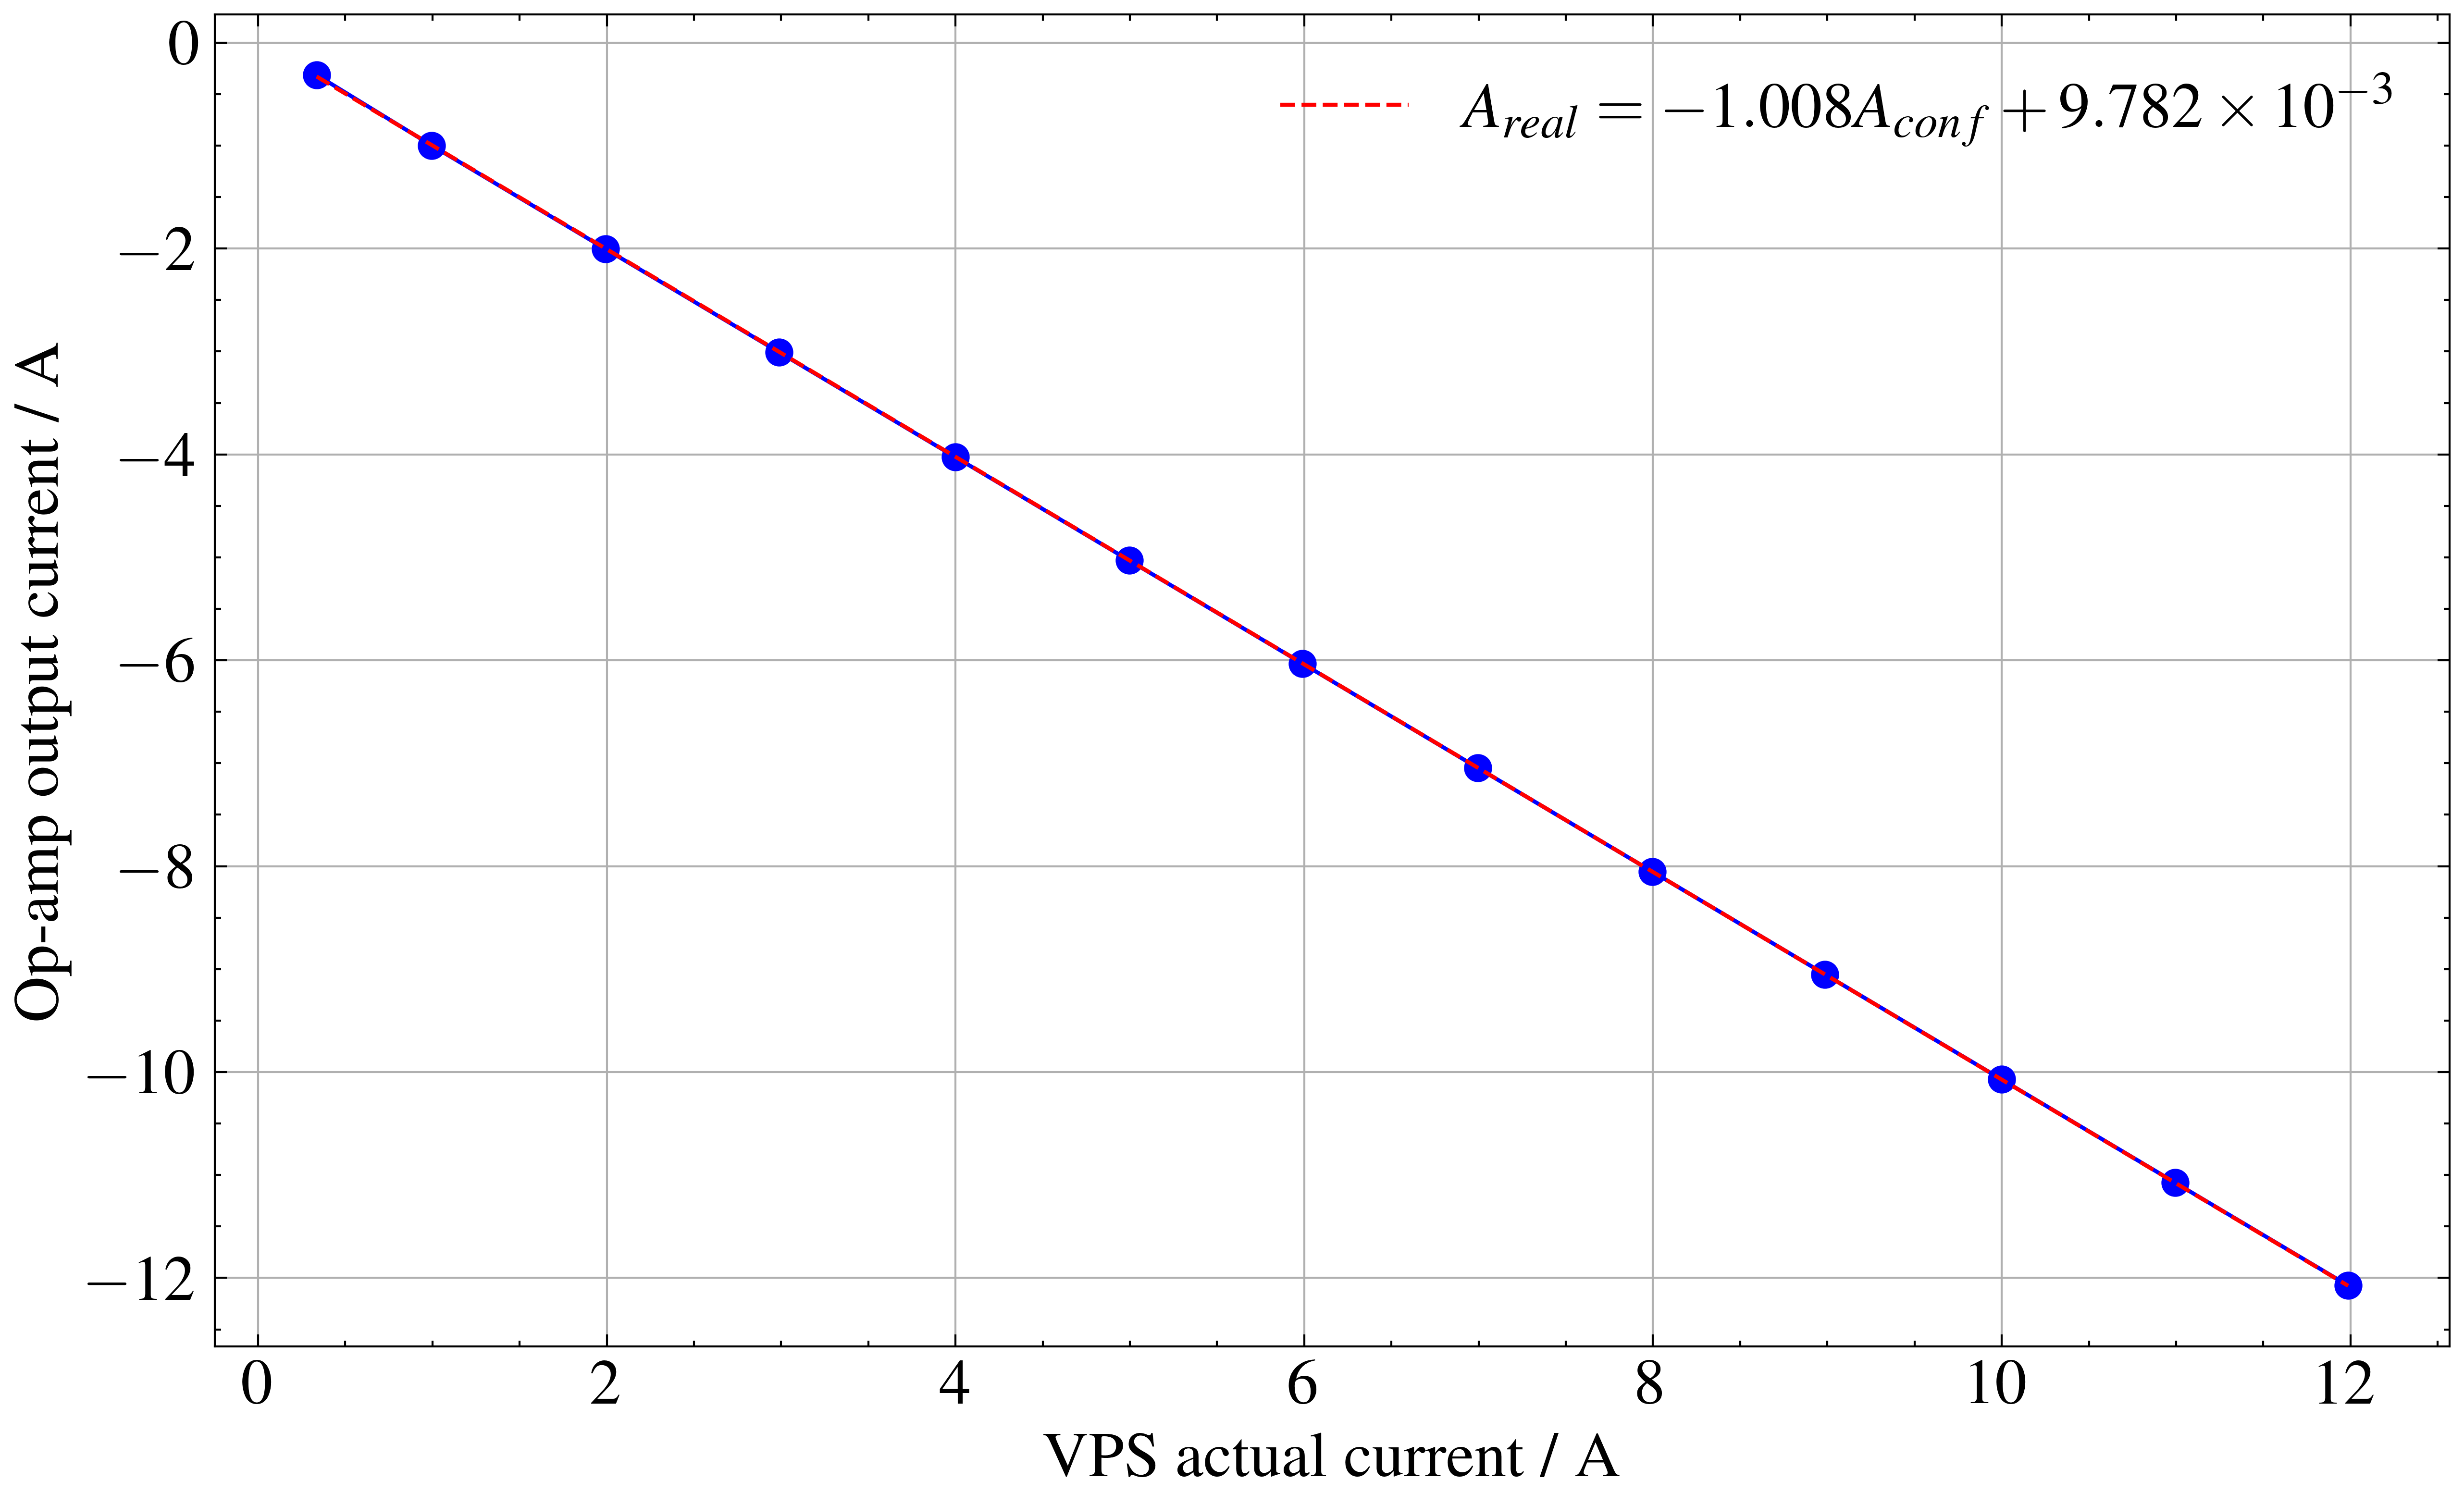
\includegraphics[width=0.6\linewidth]{src/figures/consi3/10k-vps-op-amp-with-fit.png}
	\caption{$R=\SI{10}{k\ohm}$の時のオペアンプの出力特性}\label{fig:10k-vps-op-amp-with-fit}
\end{figure}


次に$R=\SI{1}{k\ohm}$とした時を考える。
VPSの実際の出力電流に対してのオペアンプの出力電圧の図は図\ref{fig:1k-vps-op-amp-with-fit}のようになる。
\begin{figure}[!htb]
    \centering
    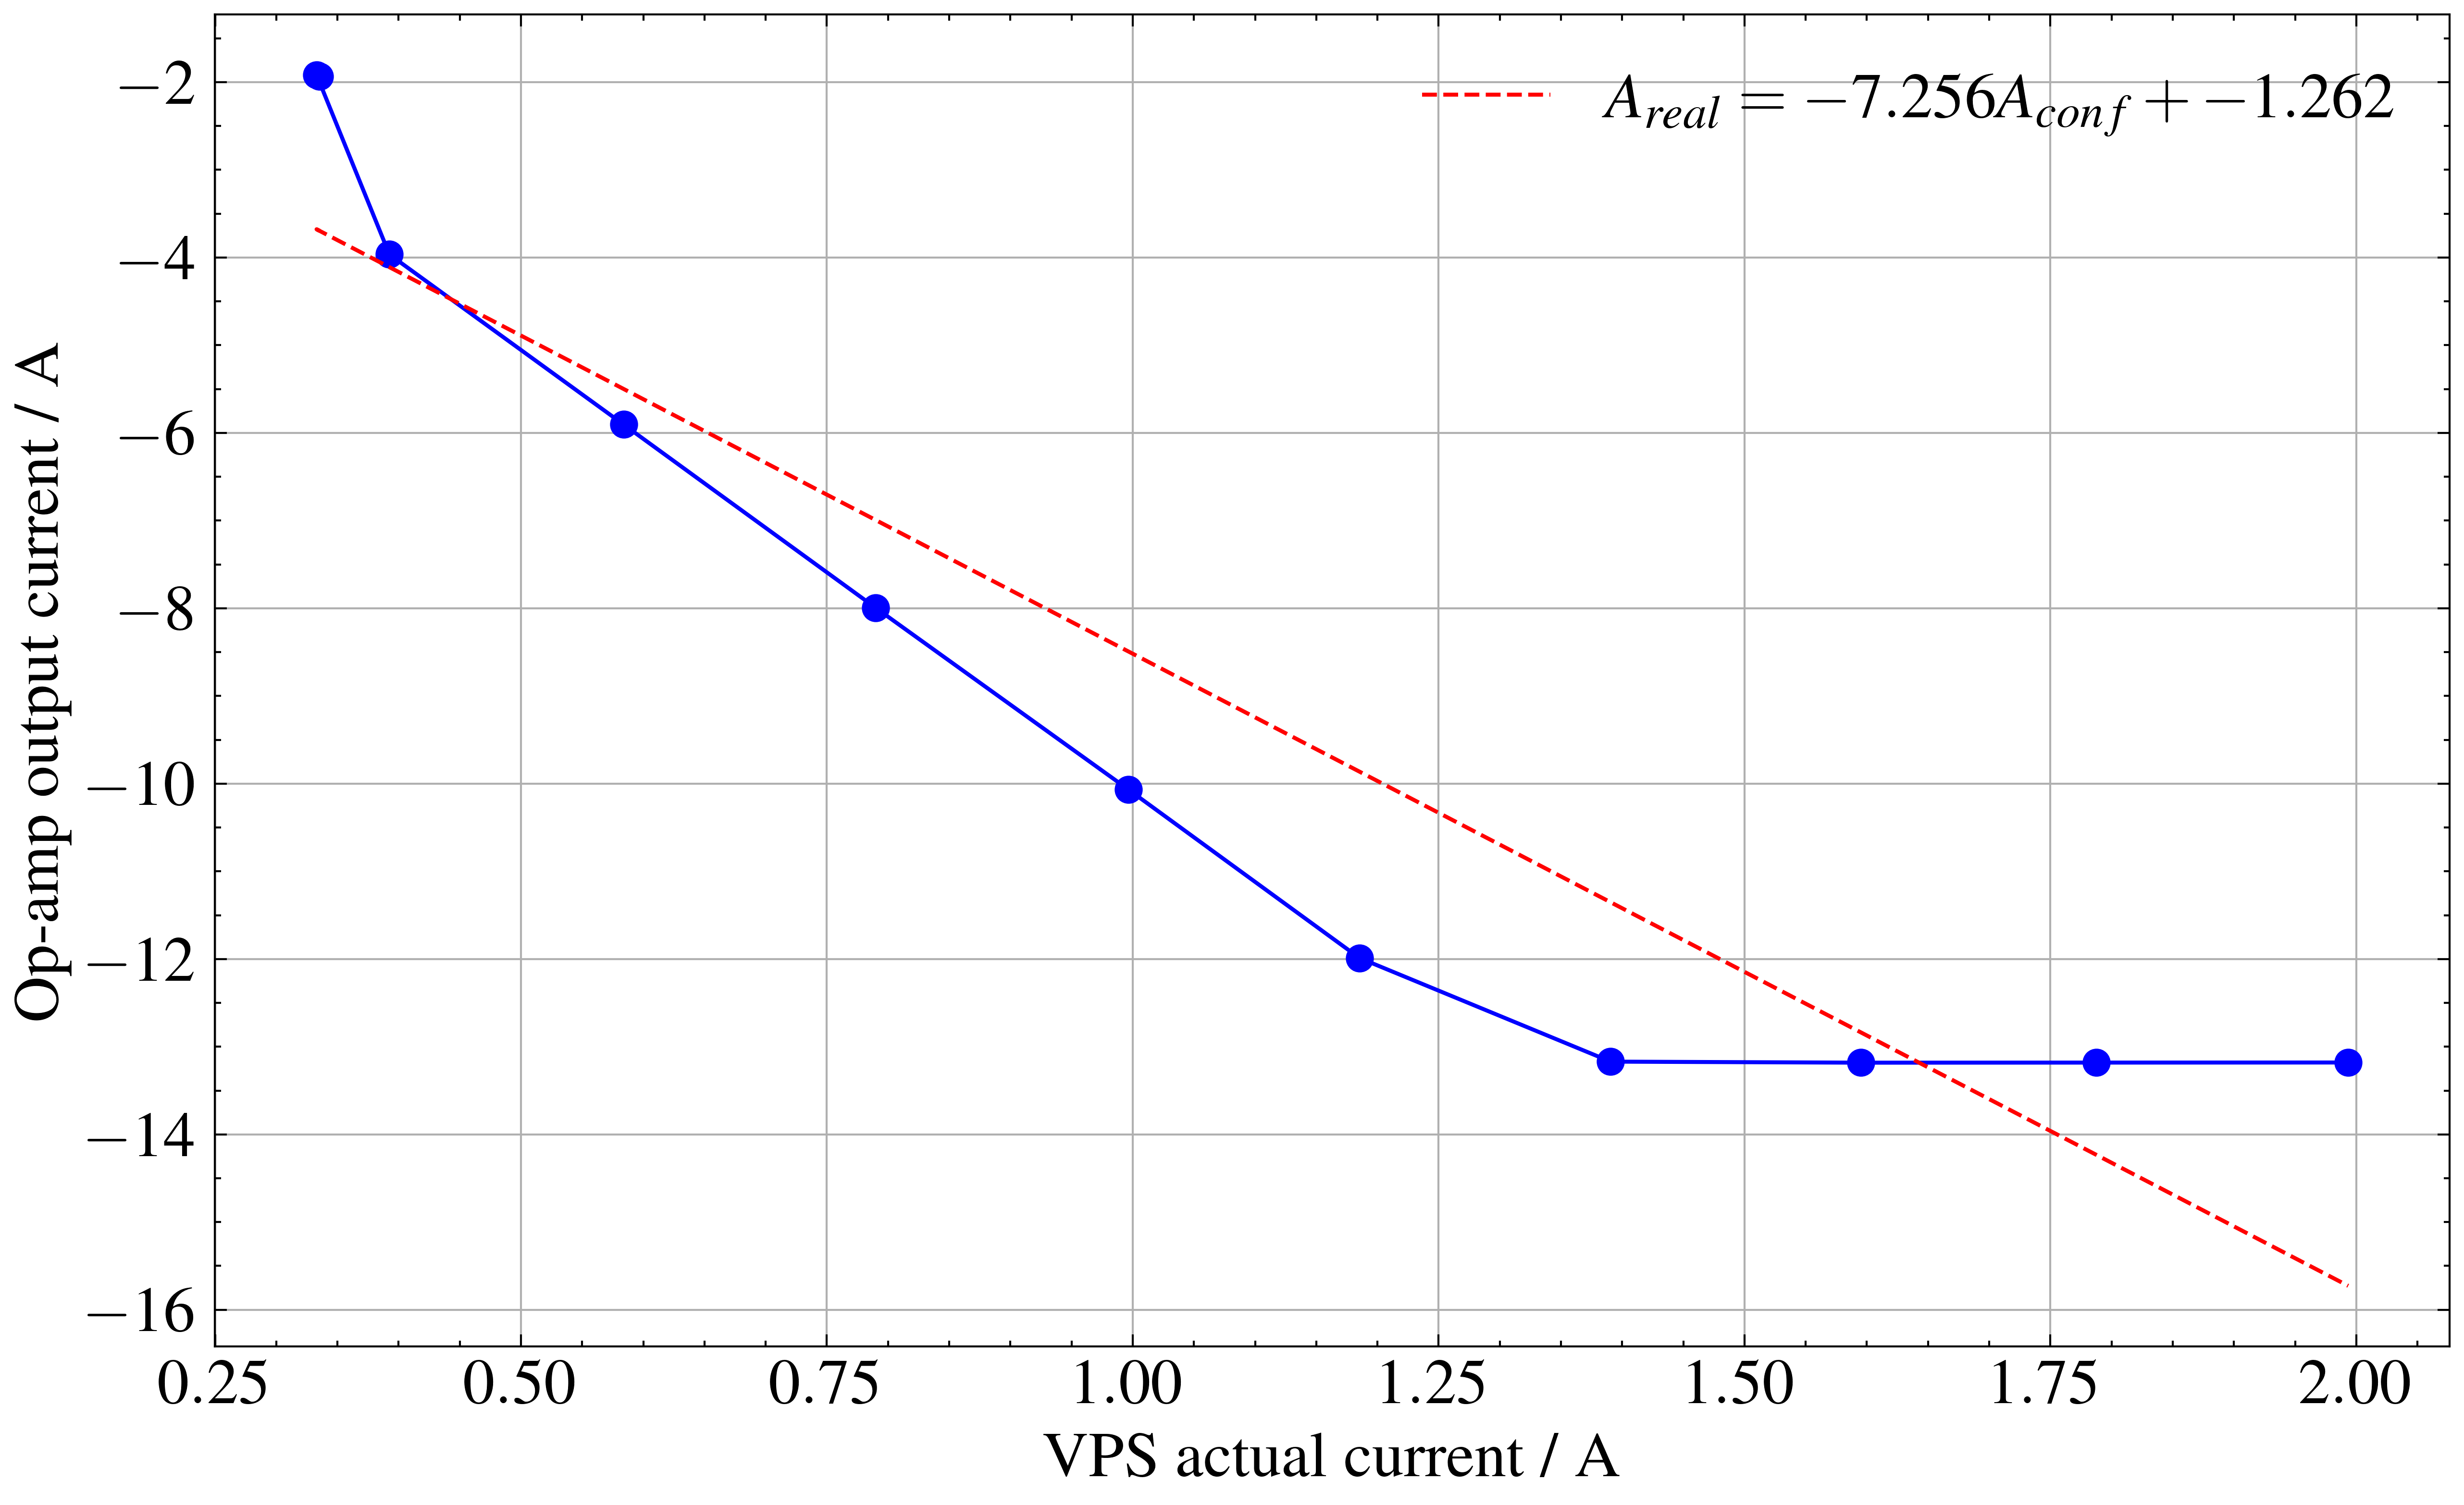
\includegraphics[width=0.6\linewidth]{src/figures/consi3/1k-vps-op-amp-with-fit.png}
    \caption{$R=\SI{1}{k\ohm}$の時のオペアンプの出力特性}\label{fig:1k-vps-op-amp-with-fit}
\end{figure}

$R=\SI{10}{k\ohm}$の考察から入力に対して$-R_0/R = -\SI{10}{k\ohm}/R$倍した出力が得られると考えられる。
一方で図\ref{subfig:exp3-10k}や表\ref{tab:exp3-1k}から入力が\SI{1.6}{A}以上では出力が\SI{-13.182}{A}から\SI{-13.180}{A}の範囲でほぼ一定値となっている。
これは、オペアンプの出力電圧$V$が負電源$V_{-}$と正電源電圧$V_{+}$の範囲、$V_- \leq V \leq V_+$しか出力できない\cite{Kossy_2024,renesas}ためである。
また、VPSの設定電流が\SI{0}{A}と\SI{0.2}{A}のときにはオペアンプの出力電圧が入力電流の-10倍程度からはズレている。
この原因として考えられるのは、\ref{subsec:consi-vps}からVPSの出力が安定していない可能性があげられる。
VPSの設定値が\SI{0.4}{A}以下の場合に実際の出力が\SI{0.3}{A}程度になっているとしたが、オペアンプの動作が正しいとすれば出力電流は\SI{0.19}{A}程度になっている可能性がある。

これらの範囲を除いて、VPSの設定電流が\SI{0.4}{A}から\SI{1.2}{A}の範囲で近似曲線を求めると、$A_{op-out}=-10.1A_{real}+\SI{1.71E-3}{}$となった。
この範囲では$R=\SI{10}{k\ohm}$のときと同様に入力に対して$-R_0/R = -\SI{10}{k\ohm}/R$倍した出力が得られている。

また、オペアンプは理想的には差動入力端子間の電圧は\SI{0}{V}であるが、実際には\SI{0}{V}にならないため、この差動入力端子間の電圧をオフセット電圧という。
このオフセット電圧は$R$に反比例する成分として図\ref{fig:10k-vps-op-amp-with-fit}と$R=\SI{1}{k\ohm}$のときは、$A_{op-out}=-10.1A_{real}+\SI{1.71E-3}{}$の$y$切片を抵抗で割った値から得られる。
$\SI{10}{k\ohm}$のときは\SI{9.78}{\micro V}、\SI{1}{k\ohm}のときは\SI{1.71}{\micro V}である。

\subsection{積分回路のボード線図と不安定性}


\end{document}
